\documentclass{article}
\usepackage[utf8]{inputenc}
\usepackage{enumerate}
\usepackage{graphicx}
\usepackage[top=2.5cm, bottom=3cm, left=2.5cm, right=2.5cm]{geometry}
\usepackage{subcaption}
\usepackage{amsmath}

\title{\textbf{LABORATORIO 2 - COMPUTACIÓN CIENTÍFICA I}}
\author{Oscar Rencoret 201173552-8 oscar.rencoret@alumnos.usm.cl \\ Ximena Rojas 201173568-4 ximena.rojas@alumnos.usm.cl}
\date{}

\begin{document}

\begin{figure}
\begin{center}

\includegraphics[width=450pt]{Logos}
\end{center}
\end{figure}

\maketitle

\section{Introducción}
El siguiente informe trata sobre los distintos métodos para la obtención de raíces, o aproximaciones a éstas, de ecuaciones en el análisis numérico de funciones reales. \\
Los métodos serán realizados con lenguaje de programación Python 3.

\section{Pequeña descripción de los experimentos}
\begin{itemize}
\item Mediante Python se desarrollarán los métodos de Bisección, Secante, Punto Fijo, Newton y Newton Modificado, y se probarán de acuerdo a las funciones dadas en el enunciado.

\item Se analizarán los errores para comprobar la tasa de convergencia existente de acuerdo a las 3 categorías: Lineal, Superlineal y Cuadrática.

\item Se mostraran aplicaciones de los métodos descritos y variantes de los mismos.
\end{itemize}

\section{Desarrollo}
\begin{enumerate}[I)]

\item Con la ayuda de Python se desarrollaron los siguientes métodos cuyos códigos se encuentran en el Anexo.
\begin{enumerate}[a)]
\item Método de la Bisección
\item Método de la Secante
\item Método del Punto Fijo
\item Método de Newton
\item Método de Newton Modificado
\end{enumerate}

\item Durante el laboratorio se verificará mediante una tabla, el tipo de convergencia por cada método desarrollado anteriormente, para cada caso estudiado.

\newpage

\item Se demuestra el poder de los métodos de Bisección y Newton para cada función propuesta:
\begin{enumerate}[(1)]

\item $f(x)=x^2-6$
\begin{itemize}
\item Método de la Bisección: La raíz encontrada es: 2.449462890625 \\
\newline
\begin{tabular}{|c|c|c|}
\hline
$\frac{e_{i+1}}{e_i}$ & $\frac{e_{i+1}}{e^{\left(\frac{1 + \sqrt{5}}{2}\right)}_i}$ & $\frac{e_{i+1}}{e^2_i}$ \\
\hline
$0.5$ & $0.43558841680114685$ & $0.4$\\
\hline 
$0.5$ & $0.6685333720787765$ & $0.8$ \\
\hline 
$0.5$ & $1.0260531555572876$ & $1.6$ \\
\hline 
$0.5$ & $1.5747681746319955$ & $3.2$ \\
\hline 
$0.5$ & $2.416926248315921$ & $6.4$ \\
\hline 
$0.5$ & $3.7094555147227104$ & $12.8$ \\
\hline 
$0.5$ & $5.693206495355222$ & $25.6$ \\
\hline 
$0.5$ & $8.737832296440896$ & $51.2$ \\
\hline
$0.5$ & $13.410669945489449$ & $102.4$ \\
\hline 
$0.5$ & $20.58245824426146$ & $204.8$ \\
\hline 
\end{tabular}
\newline
\item Método de Newton: La raíz encontrada es: -2.0000115891269745 \\
\newline
\begin{tabular}{|c|c|c|}
\hline
$\frac{e_{i+1}}{e_i}$ & $\frac{e_{i+1}}{e^{\left(\frac{1 + \sqrt{5}}{2}\right)}_i}$ & $\frac{e_{i+1}}{e^2_i}$ \\
\hline
$0.4615384615384615$ & $0.15250496289645485$ & $0.07692307692307693$\\
\hline 
$0.37113402061855666$ & $0.19775969222717277$ & $0.13402061855670103$ \\
\hline 
$0.19011295291183802$ & $0.18692325540193125$ & $0.18497872964647205$ \\
\hline 
$0.03895912941881106$ & $0.10687008190403703$ & $0.19939195018252515$ \\
\hline
\end{tabular}
\end{itemize}

\vspace{5mm}
\item $f(x)=x^5-5x^2+4,$

\begin{itemize}
\item Método de la Bisección: La raíz encontrada es: 1.0
\item Método de Newton: La raíz encontrada es: 0.8952380952380952 \\
\newline
\begin{tabular}{|c|c|c|}
\hline
$\frac{e_{i+1}}{e_i}$ & $\frac{e_{i+1}}{e^{\left(\frac{1 + \sqrt{5}}{2}\right)}_i}$ & $\frac{e_{i+1}}{e^2_i}$ \\
\hline
$0.33333333333333326$ & $0.38262419347746945$ & $0.4166666666666665$\\
\hline 
$0.1428571428571432$ & $0.32334994696153935$ & $0.5357142857142871$ \\
\hline 
\end{tabular}
\end{itemize}

\newpage

\vspace{5mm}
\item $x^4-6x^3+12x^2-10x+3$
\begin{itemize}
\item Método de la Bisección: La raíz encontrada es: 1.0
\item Método de Newton: La raíz encontrada es: 0.09280524467954615 \\
\newline
\begin{tabular}{|c|c|c|}
\hline
$\frac{e_{i+1}}{e_i}$ & $\frac{e_{i+1}}{e^{\left(\frac{1 + \sqrt{5}}{2}\right)}_i}$ & $\frac{e_{i+1}}{e^2_i}$ \\
\hline
$0.39965350110914216$ & $0.23686517815224895$ & $0.17143313720499398$\\
\hline 
$0.45610526415645397$ & $0.4764921409539741$ & $0.4895449937026915$ \\
\hline 
$1.0522085314155243$ & $1.7856726286348001$ & $2.4760776668710474$ \\
\hline 
$2.9092549818227793$ & $4.784341091241516$ & $6.506424762435749$ \\
\hline 
$0.40640029918371723$ & $0.34543111873591337$ & $0.31241570517237693$ \\
\hline 
$0.7733423892722984$ & $1.146724162058974$ & $1.4628393547474752$ \\
\hline 
$1.294195109385824$ & $2.249452950033357$ & $3.165576099496703$ \\
\hline 
$1.345538261248648$ & $1.9941304093121717$ & $2.543017221909388$ \\
\hline 
$0.5741634598040889$ & $0.708322298294319$ & $0.8064784148170612$ \\
\hline 
$10.631117640556154$ & $18.479852800748283$ & $26.00761764101839$ \\
\hline 
$0.23335369508625606$ & $0.09411819695530074$ & $0.05369791287802184$ \\
\hline 
$1.3394709793634052$ & $1.3279466632713934$ & $1.3208738741885002$ \\
\hline 
$1.7042349567011588$ & $1.410352567064023$ & $1.2546546541771368$ \\
\hline 
$0.18578352378105478$ & $0.11058910384698996$ & $0.08025506661891818$ \\
\hline 
$5.126537354279727$ & $8.635901247366128$ & $11.920162993548324$ \\
\hline 
$0.3616931290954015$ & $0.221885214704532$ & $0.16404923151121167$ \\
\hline 
$0.7167396017982846$ & $0.8243473342959782$ & $0.8987834851902163$ \\
\hline 
$0.7476869391929765$ & $1.056477376266808$ & $1.3081335251556427$ \\
\hline 
$1.032030263764267$ & $1.7453329958758037$ & $2.4149320775546963$ \\
\hline
\end{tabular}
\end{itemize}

\vspace{5mm}
\item $e^{x^2}x$
\begin{itemize}
\item Método de la Bisección: La raíz encontrada es: 1.998046875 \\
\newline
\begin{tabular}{|c|c|c|}
\hline
$\frac{e_{i+1}}{e_i}$ & $\frac{e_{i+1}}{e^{\left(\frac{1 + \sqrt{5}}{2}\right)}_i}$ & $\frac{e_{i+1}}{e^2_i}$ \\
\hline
$0.5$ & $1.1777782833303594$ & $2.0$\\
\hline 
$0.5$ & $1.8076332081976627$ & $4.0$ \\
\hline 
$0.5$ & $2.7743233693692164$ & $8.0$ \\
\hline 
$0.5$ & $4.257982273683987$ & $16.0$ \\
\hline 
$0.5$ & $6.535075630757949$ & $32.0$ \\
\hline 
$0.5$ & $10.02991810550125$ & $64.0$ \\
\hline 
$0.5$ & $15.393740315656324$ & $128.0$ \\
\hline 
\end{tabular}
\newline
\item Método de Newton: La raíz encontrada es: 0.0 \\
\newline
\begin{tabular}{|c|c|c|}
\hline
$\frac{e_{i+1}}{e_i}$ & $\frac{e_{i+1}}{e^{\left(\frac{1 + \sqrt{5}}{2}\right)}_i}$ & $\frac{e_{i+1}}{e^2_i}$ \\
\hline
$1.0338844636523943$ & $1.8043222092060913$ & $2.5455446765831233$\\
\hline 
$0.4018573053689698$ & $0.6870206008406828$ & $0.9569925858290794$ \\
\hline 
$0.030707879725016984$ & $0.09222417223187021$ & $0.1819762320931253$ \\
\hline 
$2.685339139954133e-05$ & $0.0006942647220564728$ & $0.005182199744799897$ \\
\hline
$1.921266294097965e-14$ & $3.320071315971229e-10$ & $1.3807130462750618e-07$ \\
\hline
\end{tabular}
\end{itemize}

\item
\end{enumerate}

\newpage

\item Los gráficos expuestos a continuación corresponden a las funciones señaladas anteriormente, los cuales muestran claramente las raíces reales de dichas funciones.
\begin{figure}[h]
\begin{subfigure}{.5\textwidth}
  \centering
  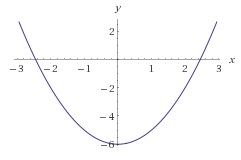
\includegraphics[width=.8\linewidth]{1}
  \caption*{Ecuación (1): Raíces: -2.4495, 2.4495}
\end{subfigure}%
\begin{subfigure}{.5\textwidth}
  \centering
  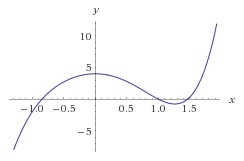
\includegraphics[width=.8\linewidth]{2}
  \caption*{Ecuación (2): Raíces: -0.84492, 1, 1.4629}
\end{subfigure}
\end{figure}
\begin{figure}[h]
\begin{subfigure}{.5\textwidth}
  \centering
  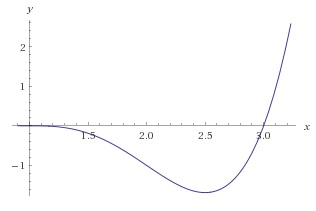
\includegraphics[width=.8\linewidth]{3}
  \caption*{Ecuación (3): Raíces: 1, 3}
\end{subfigure}%
\begin{subfigure}{.5\textwidth}
  \centering
  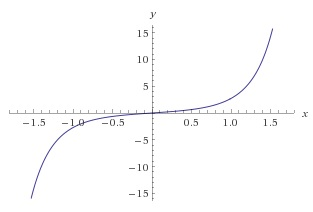
\includegraphics[width=.8\linewidth]{4}
  \caption*{Ecuación (4): Raíces: 0}
\end{subfigure}
\end{figure}

Se logra observar que en las ecuaciones (1), (2) y (3) el Método de la Bisección es el efectivo, en cambio, en la ecuación (4) el Método de Newton es el que entrega la raíz precisa. \\
Esto se debe a que el Método de Newton puede presentar diversas fallas como son la lenta convergencia de las iteraciones o cuando existe un punto crítico en $f$, es decir, la pendiente o la tangente se anulan, fallando debido a que $f'(x)=0$, lo que producirá una división por cero y no se podrá continuar.

\newpage

\item El parámetro $f(x)=cos(x)$ no se considera como input de la función debido a que es la única función sobre la que se pide actuar, se definen a mano las derivadas para términos de desarrollo: $f'(x)=-sen(x)$ y $f''(x)=-cos(x)$\\
La implementación del código para encontrar la constante \textit{c} en la expansión de \textit{Taylor} del $cos(x)$ y del código para evaluar la expansión en términos de $x \in [-0.75, .8]$. Se encuentra detallado en el Anexo.
\begin{figure}[!h]
\centering
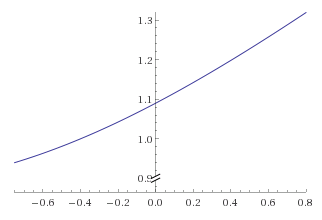
\includegraphics[width=.5\linewidth]{5}
\caption*{Gráfico de la constante \textit{c} en términos de \textit{x}}
\label{fig:my_label}
\end{figure}


\item
\begin{enumerate}[(1)]
\item En este caso se nos pide analizar el mejor valor para $M$ para que la nueva ecuación de punto fijo converge de la mejor manera, esto se logra mediante $|G'(x)|<1$\\
Para entender mejor el comportamiento de la función $G'(x)$ se hace un juego de álgebra para obtener un resultado manejable
\begin{align*}
G'(x) & = g'(x) + M(1 - g'(x))\\
G'(x) & = g'(x) + M - Mg'(x)\\
G'(x) & = g'(x)(1 - M) + M\\
\end{align*}
Desde estas ecuaciones se pueden obtener las siguientes conclusiones:
\begin{align*}
if M -> 1 & => (1 - M) -> 0\\
& => g'(x)(1 - M) -> 0\\
& => g'(x)(1 - M) -> 1\\
\end{align*}
Pero se debe considerar el hecho de que $|g'(x)| > 1$ por lo tanto:
\begin{align*}
if g'(x) > 0 AND M -> 1^{+}\\
& => (1 - M) -> 0^{-}\\
& => g'(x)(1 - M) -> 0^{-}\\
& => |g'(x)(1 - M) + M| < 1\\
\\
if g'(x) < 0 AND M -> 1^{-}\\
& => (1 - M) -> 0^{+}\\
& => g'(x)(1 - M) -> 0^{-}\\
& => |g'(x)(1 - M) + M| < 1\\
\end{align*}
Por lo que se puede concluir que el mejor valor de $M$ es alrededor de $1$ y de acuerdo al valor de $g(x)$ es de acuerdo sobre que lado se debe acercar a $1$.
\item El código de la función modificada se puede encontrar en el Anexo.
\item 
\end{enumerate}

\end{enumerate}

\section{Conclusión}
Se comprueba que es posible verificar la existencia de raíces en distintas ecuaciones mediante variados métodos, como también que en algunos casos dichos métodos no son aplicables.

\section{Referencias}
\begin{enumerate}
\item Timothy Sauer; Numerical Analysis, 2012, 2nd ed., p. 5-14
\end{enumerate}

\section{Anexo}
\begin{itemize}
\item Pregunta I:
\begin{enumerate}[a)]

\item Método de la Bisección
\begin{verbatim}
def bisection(a, b, f, tol):
    """Metodo de la biseccion para la función f(x)
    entre los intervalos a y b y con una tolerancia TOL
    listOfResult se utiliza para la deteccion del error"""
    listOfResult = []
    print("Biseccion")
    while(((b - a) / 2.0) > tol):
        c = (a + b) / 2
        listOfResult.append(c)
        if(f(c) == 0):
            break
        elif((f(a) * f(c)) <= 0):
            b = c
        else:
            a = c
    print("La raiz es: " + str(c))
    lineal(listOfResult)
    superLineal(listOfResult)
    cuadratico(listOfResult)
    return c
\end{verbatim}

\item Método de la Secante
\begin{verbatim}
def secantMethod(f, x0, x1):
    """Metodo de la secante para la funcion f(x) con los valores iniciales x0 y x1"""
    print("Secante")
    xi = x0
    xii = x1
    listOfResult = []
    listOfResult.append(xi)
    for i in range(0, limit):
        xiii = xii - ((f(xii) * (xii - xi)) / (f(xii) - f(xi)))
        if(((xii != 0) and (xi != 0) and (abs(xii - xi) / abs(xii) < tol))
        or (abs(xii - xi) == 0)):
            break
        xi = xii
        xii = xiii
        listOfResult.append(xi)
        print("Raiz encontrada: " + str(xi))
    lineal(listOfResult)
    superLineal(listOfResult)
    cuadratico(listOfResult)
    return xi
\end{verbatim}

\item Método del Punto Fijo
\begin{verbatim}
def fixedPoint(g, x0, tol):
    """Metodo de punto fijo utlizando g(x) y punto inicial x0
    Con una toleracia tol"""
    print("Punto Fijo")
    xi = x0
    listOfResult = []
    listOfResult.append(xi)
    for i in range(0, limit):
        xii = g(xi)
        if(((xii != 0) and (xi != 0) and (abs(xii - xi) / abs(xii) < tol))
        or (abs(xii - xi) == 0)):
            break
        xi = xii
        listOfResult.append(xi)
    print("Raiz encontrada: " + str(xi))
    lineal(listOfResult)
    superLineal(listOfResult)
    cuadratico(listOfResult)
    return xi
\end{verbatim}

\item Método de Newton
\begin{verbatim}
def newtonMethod(f, f_prima, x0, tol, limit):
    """Metodo de punto fijo, con la funcion de Newton
    donde f es la funcion a la que se le busca la raiz
    f_prima es la derivada de la funcion f y x0 el valor inicial
    Se considera una tolerancia tol y un limite de iteraciones lim"""
    print("Newton")
    xi = x0
    listOfResult = []
    listOfResult.append(xi)
    for i in range(0, limit):
        y = f(xi)
        yp = f_prima(xi)
        if(abs(yp) < e_mach):
            print("division por cero")
            break
        xii = xi - y/yp
        if(((xii != 0) and (xi != 0) and (abs(xii - xi) / abs(xii) < tol))
        or (abs(xii - xi) == 0)):
            break
        xi = xii
        listOfResult.append(xi)
    print("raiz encontrada: " + str(xi))
    lineal(listOfResult)
    superLineal(listOfResult)
    cuadratico(listOfResult)
\end{verbatim}

\item Método de Newton Modificado
\begin{verbatim}
def newthonModifiedMethod(f, f_prima, x0, m, tol):
    """Metodo de punto fijo, con la funcion de Newton Modificado
    donde f es la funcion a la que se le busca la raiz
    f_prima es la derivada de la funcion f y x0 el valor inicial
    y m la cantidad de raices repetidas en torno a x0
    Se considera una tolerancia tol"""
    print("Newton Modificado")
    xi = x0
    listOfResult = []
    listOfResult.append(xi)
    for i in range(0, limit):
        y = m * f(xi)
        yp = f_prima(xi)
        if(abs(yp) < e_mach):
            print("division por cero")
            break
        xii = xi - y/yp
        if(((xii != 0) and (xi != 0) and (abs(xii - xi) / abs(xii) < tol))
        or (abs(xii - xi) == 0)):
            break
        xi = xii
        listOfResult.append(xi)
    print("raiz encontrada: " + str(xi))
    lineal(listOfResult)
    superLineal(listOfResult)
    cuadratico(listOfResult)
    return xi
\end{verbatim}

\end{enumerate}

\item Pregunta II

\begin{verbatim}
def lineal(listOfResult):
	listOfErrors = []
	for i in range(0, len(listOfResult) - 1):
		listOfErrors.append(abs(listOfResult[i] - listOfResult[i+1]))
	for i in range(0, len(listOfErrors) - 1):
		if(listOfErrors[i] != 0):
			print("Lineal: " + str((float)(listOfErrors[i+1]) / listOfErrors[i]))

def superLineal(listOfResult):
	listOfErrors = []
	for i in range(0, len(listOfResult) - 1):
		listOfErrors.append(abs(listOfResult[i] - listOfResult[i+1]))
	for i in range(0, len(listOfErrors) - 1):
		if(listOfErrors[i] != 0):
			err = (float)(listOfErrors[i+1]) / ((float)(listOfErrors[i]**((1.0 + sqrt(5)) / 2.0)))
		print("Super Lineal: " + str(err))

def cuadratico(listOfResult):
	listOfErrors = []
	for i in range(0, len(listOfResult) - 1):
		listOfErrors.append(abs(listOfResult[i] - listOfResult[i+1]))
	for i in range(0, len(listOfErrors) - 1):
		if(listOfErrors[i] != 0):
			print("Cuadratico: " + str((float)(listOfErrors[i+1])/listOfErrors[i]**2))
\end{verbatim}

\item Pregunta IV
\begin{verbatim}
e_mach = 2**(-52)

def taylor_a(x, x0):
	def g(x, x0, c):
		return cos(x0) - sin(x0) * (x - x0) - cos(c) * ((x - x0) / 2.0)
	c = math.pi
	i = 0
	while((g(x, x0, c) - cos(x) > e_mach) and i < 100):
		c = g(x, x0, c)
		i += 1
	print("c = " + str(c))

def taylor_b():
	i = -.75
	while(i < .85):
		taylor_a(i, math.pi/2.0)
		i += .05

print("=============A===========")
taylor_a(math.pi, math.pi/2.0)
print("=============B===========")
taylor_b()
\end{verbatim}

\item Pregunta VI
\begin{verbatim}
def fixedPointModiefied(g, x0, tol, limit):
	"""Metodo de punto fijo modificado utilizando |g(x)|>1 y punto inicial x0
	Con una toleracia tol"""
	print("Punto Fijo")
	xi = x0
	listOfResult = []
	listOfResult.append(xi)
	for i in range(0, limit):
		xii = g(xi) - .99(xi - g(xi))
		if(((xii != 0) and (xi != 0) and (abs(xii - xi) / abs(xii) < tol)) or (abs(xii - xi) == 0)):
			break
		xi = xii
		listOfResult.append(xi)
	print("Raiz encontrada: " + str(xi))
	lineal(listOfResult)
	superLineal(listOfResult)
	cuadratico(listOfResult)
	return xi
\end{verbatim}

\end{itemize}


\end{document}


